\section{Discussion}
\label{sec:discussion}

\subsection{Main findings}
Our main finding is that through \sys's clever system design, we can achieve
privacy-preserving trigger-action execution at scale. In fact, a majority of the
most commonly used recipes can be privately executed without the use of an
expensive MPC protocol, since our design pushes predicate computations to the
trigger services. Still, \sys is general-purpose in that recipes requiring
nontrivial transformations can still be executed via MPC on the TAP.

\begin{figure}
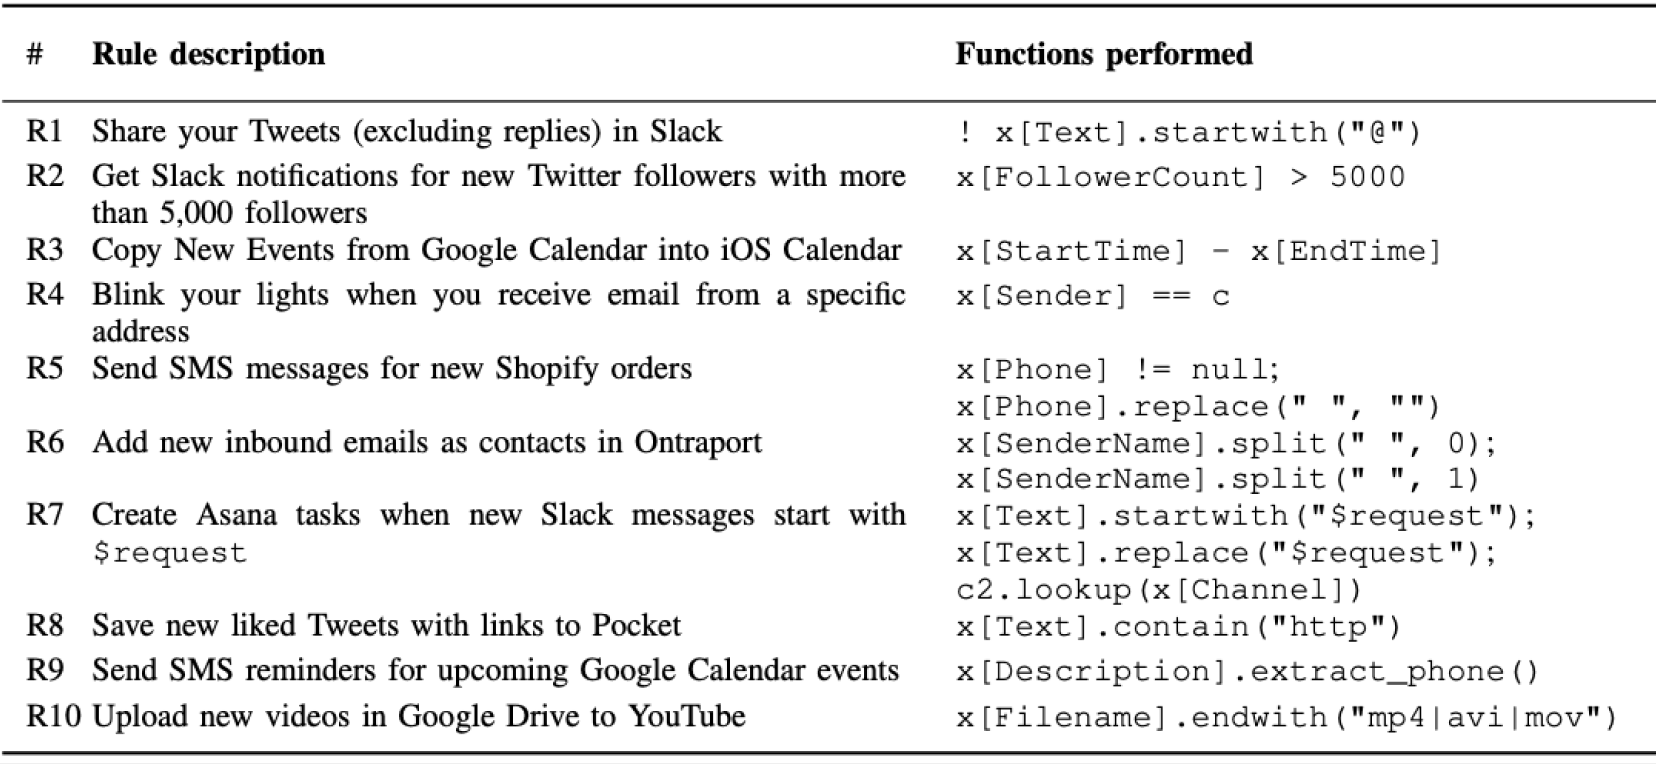
\includegraphics[width=9cm]{../graphics/etap.png}
\caption{\textbf{Selected real-world rules for our experiments from both IFTTT and Zapier from eTAP
	paper~\cite{DBLP:conf/sp/ChenCWSCF21}} We compare \sys's perfomance to that of the eTAP and therefore use the same rules eTAP used. (Figure~\ref{fig:privacy}).}
\label{fig:eTAP-rules}
\end{figure}


\subsection{Limitations}
One limitation is that \sys' design does depart from the design of existing
TAPs, whether privacy-preserving or not. Specifically, moving the computation of
predicates to trigger services does mean that they have to do more
work. However, we believe the large performance savings of not having to execute
them in MPC make this trade-off worth it. In fact, generating garbled inputs for
MPC is likely to be more expensive than simply executing the predicates
natively.

Although \sys' design is somewhat of a departure from existing TAPs, whether
privacy-preserving or not, we find that the performance gains

\subsection{Future work}

%Things we want to hide from the TAP (in order from most important to least
%important):
%\begin{itemize}[leftmargin=*]
%  \item inputs to the applet (sleep duration),
%  \item outputs to the action service (the reminder),
%  \item the applet semantics (``If sleep is under a target duration, then add a
%    reminder to Google Calendar.''), and
%  \item the services (Fitbit and Google Calendar).
%\end{itemize}\bigskip
%
%Unavoidable leakage that we might be able to leverage:
%\begin{itemize}[leftmargin=*]
%  \item The trigger service (Fitbit) already knows the inputs to the applet
%    (sleep duration).
%  \item The action service (Google Calendar) will see the outputs (the
%    reminder).
%\end{itemize}\bigskip
%
%How to hide the inputs to the applet?
%\begin{itemize}[leftmargin=*]
%  \item \emph{Multi-party computation (MPC).} The trigger service and TAP can
%    run a 2-PC to hide the inputs from the TAP.
%    \begin{itemize}
%      \item Pros: General-purpose (can compute any function over the inputs) and
%        achieves the desired notion of privacy (learns nothing about inputs
%        except what can be inferred from output)
%      \item Cons: Complicated and expensive, may require the client to be online
%        periodically, doesn't seem like the right tool for the job since the TAP
%        has no inputs, can't hide applet semantics from the TAP
%    \end{itemize}
%  \item \emph{Private function evaluation (PFE).} PFE hides both the input and
%    the function being computed~\cite{DBLP:conf/eurocrypt/MohasselS13}, though
%    it might be very slow.
%  \item \emph{Trigger service computation.} The trigger service computes the
%    conditional (i.e., ``If sleep is under a target duration'').
%    \begin{itemize}
%      \item Pros: Simple and efficient, achieves the desired notation of
%        privacy, maybe still possible to hide applet semantics from the TAP
%      \item Cons: Requires trigger service to do work (significant change from
%        how things are done today)
%    \end{itemize}
%\end{itemize}\bigskip
%
%How to hide the outputs of the applet?
%\begin{itemize}[leftmargin=*]
%  \item \emph{Encrypt to action service.} Need to know more about how actions
%    work. Are they static (i.e., send message to action service)? Are they
%    dynamic (i.e., inject part of input into message to action service)?
%    \begin{itemize}
%      \item Note: This is expensive to do in MPC, but easy otherwise (each
%        action service has public key, and client installs action rule with TAP
%        that encrypts the message to the action service).
%    \end{itemize}
%\end{itemize}\bigskip
%
%How to hide the applet semantics?
%\begin{itemize}[leftmargin=*]
%  \item \emph{Trigger service talks to action service directly.} Trigger service
%    learns actions service, have to give OAuth tokens to trigger service (some
%    trigger services might be sketchy), trigger service has to do more work.
%  \item \emph{Trigger service computation + encrypt to action service.}  Client
%    generates fresh key pair and installs public key with trigger service and
%    secret key with action service. Trigger service encrypts true/false to
%    action service, and proxies through TAP. Action service decrypts result,
%    uses oblivious transfer to retrieve action output.
%\end{itemize}\bigskip
%
%How to hide the services?
%\begin{itemize}[leftmargin=*]
%  \item This is probably too hard (probably have to add proxies).
%\end{itemize}\bigskip
%
%\paragraph{Protocol flow.}
%The client installs an applet as follows:
%\begin{enumerate}[leftmargin=*]
%\item The client generates a key pair $(\sk, \pk)$.
%\item The client sends $\sk$ to the action service and $\pk$ to the trigger
%  service.
%\item On the trigger service, the client installs a rule with an action
%  encrypted to the action service.
%\item On the TAP, the client configures forwarding/polling rules between trigger
%  service and action service.
%\end{enumerate}
%Applets run as follows:
%\begin{enumerate}[leftmargin=*]
%\item The trigger service evaluates the rule, and encrypts the resulting bit to
%  the action service. If the result is 1, then the trigger service sends the
%  encrypted action to the TAP. Otherwise, if the result is 0, then the trigger
%  service sends an encryption of zeros to the TAP.
%\item The TAP forwards the message to the action service.
%\item The action service decrypts the message and executes the action if valid.
%\end{enumerate}
%
%\bigskip
%Questions to think about:
%\begin{itemize}[leftmargin=*]
%\item How to add integrity?
%\item Xiangchang Mi et al. paper creates a service on IFTTT to see the interaction from both channels,
%while testing we would need to the same thing and see how much we can learn about the recipe or
%other things.
%\item same paper found the delays between triggers and actions because of IFTTT's long polling interval (sometimes up to 15min, usually 1-2min) -- try to see if we can find what is the IFTTT's polling interval and if we can improve it without traffic overload?
%\item same paper: when multiple applets run sequentially and concurrently, they form explicit and implicit infinite loops, wasting or damaging devices. How can we improve this?
%\end{itemize}
